% This file was created with tikzplotlib v0.10.1.
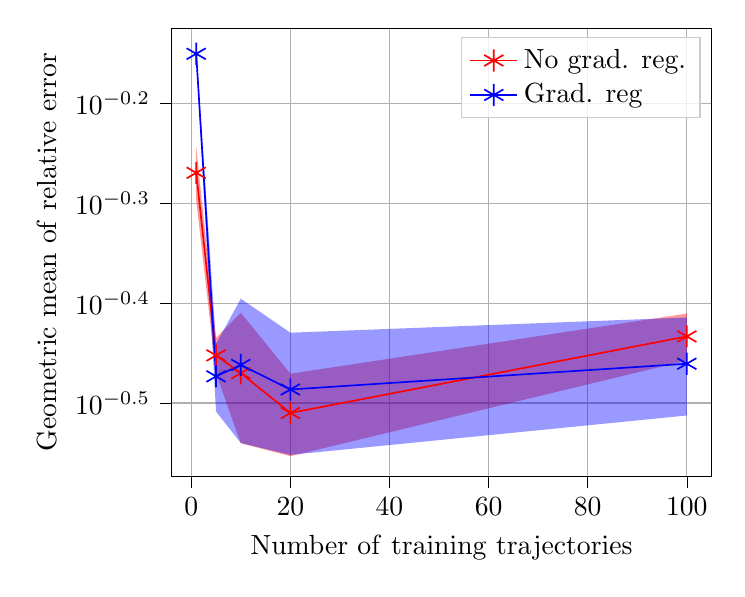
\begin{tikzpicture}

\definecolor{darkgray176}{RGB}{176,176,176}
\definecolor{lightgray204}{RGB}{204,204,204}

\begin{axis}[
legend cell align={left},
legend style={fill opacity=0.8, draw opacity=1, text opacity=1, draw=lightgray204},
log basis y={10},
tick align=outside,
tick pos=left,
x grid style={darkgray176},
xlabel={\(\displaystyle \mathrm{Number \ of \ training \ trajectories }\)},
xmajorgrids,
xmin=-3.95, xmax=104.95,
xtick style={color=black},
y grid style={darkgray176},
ylabel={\(\displaystyle \mathrm{Geometric \ mean \ of \ relative \ error }\)},
ymajorgrids,
ymin=0.266942476442463, ymax=0.749832116349196,
ymode=log,
ytick style={color=black}
]
\path [fill=red, fill opacity=0.4, semithick]
(axis cs:1,0.570241689624135)
--(axis cs:1,0.504474483117348)
--(axis cs:5,0.338357373021068)
--(axis cs:10,0.288190658397173)
--(axis cs:20,0.279773229275691)
--(axis cs:100,0.348821336887377)
--(axis cs:100,0.388578507231413)
--(axis cs:100,0.388578507231413)
--(axis cs:20,0.338310911935988)
--(axis cs:10,0.389291486552578)
--(axis cs:5,0.367432942562177)
--(axis cs:1,0.570241689624135)
--cycle;

\path [fill=blue, fill opacity=0.4, semithick]
(axis cs:1,0.715443870639624)
--(axis cs:1,0.698573508358372)
--(axis cs:5,0.310079630122696)
--(axis cs:10,0.288415372061087)
--(axis cs:20,0.280623604111376)
--(axis cs:100,0.307269293148806)
--(axis cs:100,0.385109020949594)
--(axis cs:100,0.385109020949594)
--(axis cs:20,0.371861419913497)
--(axis cs:10,0.402089649881176)
--(axis cs:5,0.362463126008537)
--(axis cs:1,0.715443870639624)
--cycle;

\addplot [semithick, red, mark=asterisk, mark size=4, mark options={solid}]
table {%
1 0.537358164787292
5 0.352895140647888
10 0.338741093873978
20 0.309042096138
100 0.368699908256531
};
\addlegendentry{No grad. reg.}
\addplot [semithick, blue, mark=asterisk, mark size=4, mark options={solid}]
table {%
1 0.70700865983963
5 0.336271375417709
10 0.345252513885498
20 0.326242476701736
100 0.346189230680466
};
\addlegendentry{Grad. reg}
\end{axis}

\end{tikzpicture}
